% !TEX TS-program = arara
% arara: xelatex: { synctex: on, options: [-halt-on-error] } 
% % arara: biber
% % arara: texindy: { markup: xelatex }
% %% arara: makeglossaries
% % arara: xelatex: { synctex: on, options: [-interaction=batchmode, -halt-on-error] }
% % arara: xelatex: { synctex: on, options: [-interaction=batchmode, -halt-on-error]  }
% % arara: clean: { extensions: [ aux, log, out, run.xml, ptc, toc, mw, synctex.gz, ] }
% % arara: clean: { extensions: [ bbl, bcf, blg, ] }
% % arara: clean: { extensions: [ glg, glo, gls, ] }
% % arara: clean: { extensions: [ idx, ilg, ind, xdy, ] }
% % arara: clean: { extensions: [ plCode, plData, plMath, plExercise, plNote, plQuote, ] }
%-----------------------------------------------------------------
\documentclass[11pt]{PalisadesLakesBook}
% \geomHDTV
% \geomLandscape
\geomHalfDTV
\geomPortraitOneColumn
%-----------------------------------------------------------------

%\AsanaFonts % misssing \mathhyphen; less on page than Cormorant/Garamond
%\CormorantFonts % light, missing unicode greek
\EBGaramondFonts % fewest pages
%\ErewhonFonts
%\FiraFonts % tall lines, all sans, much less per page, missing \in?
%\GFSNeohellenicFonts 
%\KpFonts
%\LatinModernFonts
%\LegibleFonts
%\LibertinusFonts
%\NewComputerModernFonts
%\STIXTwoFonts
%\BonumFonts % most pages
%\PagellaFonts

%\ScholaFonts
%\TermesFonts
%\XITSFonts

%-----------------------------------------------------------------
\togglefalse{plMath}
\togglefalse{plCode}
\togglefalse{plData}
\togglefalse{plNote}
\togglefalse{plExercise}
\togglefalse{plQuote}
\togglefalse{printglossary}
\togglefalse{printindex}
%-----------------------------------------------------------------
\title{Notes on typography}
\author{John Alan McDonald 
(palisades dot lakes at gmail dot com)}
\date{draft of \today}
%-----------------------------------------------------------------
\begin{document}
\maketitle
\PalisadesLakesTableOfContents{7}
%-----------------------------------------------------------------
\def\sharedFolder{../../shared/}
%-----------------------------------------------------------------
\begin{plSection}{Introduction}

This is a collection of notes on font design,
typesetting (both for text and mathematics),
and possibly related layout problems. 
Partially notes on reading; 
partially my own work-in-progress analysis and implementation.
%-----------------------------------------------------------------
\begin{plSection}{Organizing thoughts}

\begin{itemize}

\item Better handwriting, rather than reproduce the best
traditional lead typesetting.

\item \emph{Question:} Compare evolution from handwriting to 
typesetting (including font development) for
math and 
汉字/\allowbreak 漢字/\allowbreak Hànzì/\allowbreak Kanji/\allowbreak Hanja/\allowbreak \mbox{Chữ Nôm}?\\
\citeAuthorYearTitle{MoteChu:1989:CalligraphyEABook}\\
\citeAuthorYearTitle{Kraus:1991:BrushesWithPower}
 
\item What could I (or somebody) do better
if I (they) were going to replace \TeX, \LaTeX, etc.


\end{itemize}
%-----------------------------------------------------------------
\end{plSection}%{Organizing thoughts}
%-----------------------------------------------------------------
\end{plSection}%{Introduction}
%-----------------------------------------------------------------
\begin{plSection}{Reading}
%-----------------------------------------------------------------
\begin{plSection}{Knuth}

\citeAuthorYearTitle{Knuth:1979:MathTypography}

\citeAuthorYearTitle{BeetonPalais:2016:CMT}

\citeAuthorYearTitle{Smith:2017:MathTypography}.

\end{plSection}%{Knuth}
%-----------------------------------------------------------------
\begin{plSection}{Microsoft}


\end{plSection}%{Microsoft}
%-----------------------------------------------------------------
\begin{plSection}{Math style guides}
%-----------------------------------------------------------------
\begin{plSection}{American Mathematical Society}

\citeAuthorYearTitle{Swanson:1999:MathIntoType}

\citeAuthorYearTitle{LetourneauSharp:2017:AMSStyleGuide}

\end{plSection}%{American Mathematical Society}
%-----------------------------------------------------------------
\begin{plSection}{London Mathematical Society}

\citeAuthorYearTitle{RoddTornqkvist:2009:LMSStyleGuide}

Seems aimed at traditional kind of typesetting:
paper(?) copy marked in pencil(?)  
passed on to typesetter for formatting.

Interesting typo? on p $21$: ``$\theta$ vs $\mathscr{V}$''

Useful list of ``mathematical statement'' types.

Slanted fonts for emphasis; no italic in text;
math variables italic/roman by author's choice.

Latex commands used to communicate with typesetter.


\end{plSection}%{London mathematical Society}
%-----------------------------------------------------------------
\begin{plSection}{Oxford University Press}

\citeAuthorYearTitle{ChaundyBarrettBatey:1954:PrintingMathematics}

\end{plSection}%{Oxford University Press}
%-----------------------------------------------------------------
\end{plSection}%{Math style guides}
%-----------------------------------------------------------------
\begin{plSection}{Font design}
%-----------------------------------------------------------------
\begin{plSection}{Noordzij}

\citeAuthorTitle{Devroye:2014:Noordzij}

\citeAuthorTitle{Middendorp:2019:Noordzij}

\end{plSection}%{Noordzij}
%-----------------------------------------------------------------
\begin{plSection}{Rhatigan}
%-----------------------------------------------------------------
\begin{plSection}{The Monotype 4-line system}

\citeAuthorYearTitle{Rhatigan:2007:Monotype4Line}

A 38 page essay reviewing the Monotype (UK)
4-line system for mathematics typesetting.
The essay doesn't put much attention on the chronology
(probably covered well in the references),
but it appears that the development
began some time shortly after the end of WWII,
with the first installed system in June of 1958.
This appears to be roughly contemporaneous with
the development of the Monotype Filmsetter,
which (I'm guessing) made the hot lead type machines 
obsolete.~\cite{Eye:2012:MonotypeTimeline}

\emph{Question:} What, if anything, can we learn from the
4-line system that is relevant to digital typesetting
of mathematics?

\emph{Question:} To what extent did the limitations of
hot lead typesetting, of any kind, 
fail to reproduce math notation as practiced by mathematicians?
To what extent are these (now unnecessary) restrictions
carried over (perhaps unconsciously) into digital typesetting,
and webpage layout?

\begin{plQuote}
{\citeAuthorYearTitle[p.~11]{Rhatigan:2007:Monotype4Line}}
{PostwarMonotype}
As it resumed production in the wake of the war,
Monotype found itself struggling to meet its customers'
demands for parts and equipment. 
In this climate of an uncertain return to economic stability,
it makes sense that the company would choose to develop
technology such as the 4-line system that adapted to its existing
equipment and working methods, 
rather than solutions that would make unrealistic demands
on the company's ability to devise and manufacture 
new kinds of equipment altogether. 
\end{plQuote}

Idea seems to be 4 half-lines, with extra 2pt spaces between the 
upper and lower pairs.
Half-lines wide (high) enough for sub/super script chars;
2 half-lines (roughly?) equivalent to normal char height, 
normal line of text.
The extra 2pt space is to allow for clean horizontal rules in
fractions.
Examples (fig 8, 9) show integrals $\int$ 
taking advantage of 
available double line height, but not sums $\sum$,
and the sum readability suffers.

Figures 9 and 10 compare a traditional setting with 4-line result,
and, although neither looks good to me,
the 4-line is a little better,
though that's primarily because the greek letters 
in the traditional setting are too small,
as mentioned in the captions.
In figure 10, however, although the kerning of 
$L^2$ is a bit better, other spacing is screwed up:
\begin{itemize}
\item $\sin^2 \,\omega$ rather than $\sin^{2}\!\omega$ or, even better, 
 $\textrm{sin}^{2}\!\left(\omega\right)$
\item $v_{\,1}\;,\;v_{2}$ rather than $v_{1},v_{2}$
\item $\sum\,'$ rather than $\sum^{'}$
\end{itemize}

Developed together with Times 4-line Mathematics Series 569 font
derived from Times New Roman Series 327. 

\begin{plQuote}{\citeAuthorYearTitle[p.~21]{Rhatigan:2007:Monotype4Line}}
{}
Planning the correct keying sequence is a critical part of the
training for a keyboard operator setting maths.
Rather [than] reading through manuscript text 
in a linear fashion,
the operator needs to examine each equation in a manuscript,
determine how much of it can be set mechanically,
and then how the characters and symbols within that equation
should be positioned within the 4 available lines. 
\textit{(See figure 13.)}
For any characters that cannot be set in line with the others
(characters larger than 12 points, for example,
or additional symbols that could not be fit into the matrix case),
spaces of equal width (removed by the compositor later)
are needed to hold their position for justification.
\end{plQuote}

\begin{plQuote}{\citeAuthorYearTitle[p.~25]{Rhatigan:2007:Monotype4Line}}
{}
\ldots increased the speed of maths composition 
by an average of 26 percent.
\end{plQuote}

\begin{plQuote}{\citeAuthorYearTitle[p.~25]{Rhatigan:2007:Monotype4Line}}
{}
Series 569 and the principles of the 4-line layout 
were even adapted for Monophoto---Monotype's 
filmsetting technology---and their relevance carried on 
until the digital era demand other solutions 
for setting mathematics.
\end{plQuote}

\emph{Conclusions:}
Seems fundamentally limited. 
No doubt a reasonable economic compromise given the technology of
the time, but not a model for high-resolution digital typesetting.

For additional history, see
\citeAuthorYearTitle{Smith:2017:MathTypography}.

\emph{Note:} \TeX was invented, at least in part, 
to reproduce the perceived superior quality 
of 4-line Monotype setting
in the first edition of Knuth, The Art of Computer Programming
(see \citeAuthorYearTitle{BeetonPalais:2016:CMT}).

\end{plSection}%{The Monotype 4-line system}
%-----------------------------------------------------------------
\begin{plSection}{Gina}

\begin{plSection}{\citeAuthorYearTitle{Rhatigan:2007:GinaPractice}}

A 40 page essay on the experience of developing the type family
Gina.

\begin{plQuote}{\citeAuthorYearTitle[p.~1]{Rhatigan:2007:GinaPractice}}{}
This document is more an analysis of that process of discovery
[for designing a typeface]
than a guide to designing type.
The missteps and the inefficiencies discussed, though, 
point the way to more sound methods for 
Gina's own future development as well as that of other typefaces.
\end{plQuote}

Section 2.1: Gina intended as a serif typeface 
``matching math to the text''.

(\emph{Comment:} Not a desirable goal for me, depending
on what ``matching'' means.
Important to easily distinguish math notation from normal text,
especially when mixed. 
Analogy to 漢字\allowbreak ひらがな\allowbreak カタカナ\allowbreak romaji
(kanji hirgana katakana romaji) pre-parsed Japanese text?)


\begin{plQuote}{\citeAuthorYearTitle[p.~3]{Rhatigan:2007:GinaPractice}}{}
Gina was originally conceived as a serif typeface family
for textbooks and other technical publications that may include
equations, chemical formulas, tables, and other combinations of
text, numerals, and symbols.
Material like this requires type that will facilitate long dense
passages of text, but it must also feature glyphs with enough
individual clarity that they can be recognized outside of typical
word shapes, such as in mathematical or chemical formulae.
\end{plQuote}

\emph{Comment:} 
Compare to \citeAuthorYearTitle{Braille:2021:AtkinsonHyperlegible},
\citeAuthorYearTitle{DobieScottScott:2021:AtkinsonHyperlegible}.

References \citeAuthorYearTitle{Bouche:2003:DiversityMathFonts}.

Figure 4 compares Gina to more conventional set of fonts:
\begin{itemize}
  \item Gina digits too small in $2i$ and $1.0\,g$, 
  should either descend below baseline ot rise above x-height.
  \item Gina $3/4$ is too small.
  \item Conventional setting seems to use slanted rather 
  than italic capitals, which I find easier to read, less cramped.
  \item Gina's rounder italic $\mathit{a}$ is better; 
  probably upright sans would be better still.
  \item Gina seems to get heavier as Adobe Reader zooms in?
  Conventional setting feels like the same weight regardless. 
\end{itemize}

Design process began, in class, with pencil sketches on paper,
starting from Morris Fuller Benton's New Century 
Schoolbook~[p.~7].
Pencil sketches scanned and traced~[p.~8, fig.~7] 
in FontLab Studio 5.0.2~\cite{FontLab:2021}.

\begin{plQuote}{\citeAuthorYearTitle[p.~9]{Rhatigan:2007:GinaPractice}}{}
Concentrating on the outlines often resulted in clear details
but distorted characters overall.
Calligraphy exercises, attempted without much experience 
using a broad nib pen, resulted in letters too crude
to be helpful. Drawing directly in FontLab was just as awkward
at this beginning stage.

A technique of jotting down some key positions on paper
before connecting parts of the contours---building up from gestural
lines and basic proportions to overall shapes 
and then on to finer elements, 
refining the good lines and slowly eliminating the bad ones---was
somewhat more helpful.
Rather than collage of connected details,
these drawings produced an overall \emph{sense of mass} 
and \emph{relationships between parts.}
Made with larger motions fo the arm and the hand,
the straight lines had more \emph{tension}
and the curves had more \emph{swing} 
the the slower, more deliberate contour drawings.
[\emph{Emphasis} added.]
\end{plQuote}

\emph{Question:}
Can we quantify \emph{mass} and \emph{relationships},
and optimize \emph{tension} and \emph{swing}?

Section 3.3: experience with non-Latin (Indic and Greek) 
scripts helpful~[figs.~8,~9]. Broad nibbed pen for Devanagari
and unspecified ``rounder tool'' for greek.

\begin{plQuote}{\citeAuthorYearTitle[p.~11]{Rhatigan:2007:GinaPractice}}{}
The insights from these two workshops into the relationship
of action and form led to some different sketching
techniques---particularly the use of pen and ink 
to experiment with discrete shapes as well as entire 
letters---that fed into Gina's eventual design.
\textit{(See figures 10 and 11.)}
They also led to a means of distinguishing similar forms
in the roman, italic, and Greek glyphs:
using the writing tradition to guide the overall look
of each set of shapes in a slightly different direction.
\end{plQuote}

Figure 10 shows ideal singularities the result from two pencils
tied together to simulate and edged pen: the two curves cross over
as the 'pen' changes direction --- invisible 
with an actual edged pen because the ink path never goes 
completely to zero width.

\emph{TODO:} Work this out in a little more detail. 
Cross-over happens the direction of motion passes thru parallel 
to the pen edge.

\emph{TODO:} 
Compare this to \citeAuthorYearTitle{Noordzij:2006:TheStroke}.

\emph{TODO:} the below in not quite right.
Want something that can be filled to simulate ink.
That requires connecting the left and right curves
at extrema, in some sense.

\emph{TODO:} must be some way to define the central path just once? 
\begin{plDiagram}{Stroking with an edged pen}{}
\center
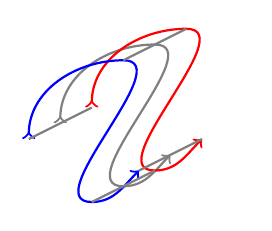
\begin{tikzpicture}
\path[>->,thick,gray,draw] (0mm,0mm) 
to [out=90,in=180] (12mm,10mm)
to [out=0,in=180] (8mm,-8mm) 
to [out=0,in=-135] (14mm,-4mm) ;
\path[>->,thick,red,xshift=4mm,yshift=2mm,draw]
 (0mm,0mm) 
to [out=90,in=180] (12mm,10mm)
to [out=0,in=180] (8mm,-8mm) 
to [out=0,in=-135] (14mm,-4mm) ;
\path[>->,thick,blue,xshift=-4mm,yshift=-2mm,draw] 
(0mm,0mm) 
to [out=90,in=180] (12mm,10mm)
to [out=0,in=180] (8mm,-8mm) 
to [out=0,in=-135] (14mm,-4mm) ;
% pen edge sampled at control points
\path[thick,gray,draw] 
(-4mm,-2mm) to (0mm,0mm) to (4mm,2mm) ; 
\path[thick,gray,xshift=12mm,yshift=10mm,draw] 
(-4mm,-2mm) to (0mm,0mm) to (4mm,2mm) ; 
\path[thick,gray,xshift=8mm,yshift=-8mm,draw] 
(-4mm,-2mm) to (0mm,0mm) to (4mm,2mm) ; 
\path[thick,gray,xshift=14mm,yshift=-4mm,draw] 
(-4mm,-2mm) to (0mm,0mm) to (4mm,2mm) ; 
\end{tikzpicture}
\end{plDiagram}

\begin{plQuote}{\citeAuthorYearTitle[fig.~11]{Rhatigan:2007:GinaPractice}}{}
\ldots a closer look at more types 
by Dwiggins made it clear he was manipulating details to provide 
an even stronger sense of the pen stroke in small point sizes.
\end{plQuote}

Figure 17 shows a comparison of varying extender lengths
generated by FontLab, using two 'master' fonts generated by hand,
with one interpolation and two extrapolations.

\begin{plQuote}{\citeAuthorYearTitle[p.~21]{Rhatigan:2007:GinaPractice}}{}
The italic and Greek glyphs took cues from a tradition of
written forms just as Gina's roman did.
Although none of the styles would slavishly follow calligraphic 
shapes,
using these three distinct writing styles as a point of departure
for the design provided a means to distinguish the forms from one
another in text.
\end{plQuote}

Section 5: experience with roman made it possible
to draw italic and greek directly in FontLab.

Section 5.1: experiments with italic slope, by slanting roman.

Fig. 23: some greek pangrams~\cite{wiki:Pangram} 
to use in font testing.

Section 5.3: designing figures to match (roman? italic?)
more difficult than expected.

Fig 25: blocks of figures and symbols used to even out apparent
weight, to merge visually into other text---but that's probably
the wrong goal: certainly math symbols shouldn't disappear into
normal text, and maybe not numbers either.
Also, tested operators are much too small.

Fig.27: spacing test, unclear if the test was done at normal size
or at thumbnail size (thumbnail test would be wrong). Also. seems
like goal is even texture for mixture of math, greek, italic, 
roman; not likely the right goal.

Section 6: extended character set required 
``more systematic handling'' (automation?).
Not clear if he succeeded.
``{\ldots} most difficult aspect{\ldots}was constructing test
documents in Adobe InDesign{\ldots}''. 

(Why Adobe InDesign? 
Would {\LaTeX} help?
Software to find suitable, real examples of extended char set use 
in web pages and documents, pdf or something else?) 

(Reviewing lots of docs by eye seems difficult.
Might help to have a fixed test set plus continued sampling
of new docs.
Any possibility of partial automation, eg, variation in blurred
image, local 2d spectra.
Experimenting with image transforms that expose layout issues 
to the eye might be a way to find objective functions that
could be used for automated optimization of glyph design
and page layout.) 

Section 7: Future development. Gina unfinished, esp italic,
and math barely started.

\begin{plQuote}{\citeAuthorYearTitle[p.~31]{Rhatigan:2007:GinaPractice}}{}
This version of Gina was optimised for common desktop publishing
software (primarily so testing could be restricted to a 
manageable set of technical issues). 
In reality those are not the tools commonly used to typeset 
mathematics, and in the end Gina will probably need to be
re\"{e}ngineered for a different production environment.
\end{plQuote}
 
\begin{plQuote}{\citeAuthorYearTitle[p.~33]{Rhatigan:2007:GinaPractice}}{}
Many repetitive tasks such as repositioning components or
adjusting the stem height of new optical sizes are instructional 
the first few times,
but better handled by automation 
once the principles are understood.

{\ldots}
Learning to perceive and manipulate subtle variations in shape,
in weight, and in proportion was the most difficult part 
of this past year.
{\ldots} Learning how to discern---and hopefully enhance---the
relationships within a set of shapes became
an entirely new way to understand not only typefaces,
but also typography in a broader sense.
\end{plQuote}
 
 

\end{plSection}%{\citeAuthorYearTitle{Rhatigan:2007:GinaPractice}}
%-----------------------------------------------------------------
\begin{plSection}{\citeAuthorYearTitle{Rhatigan:2007:GinaSpecimen}}

Tabular oldstyle figures (digits) are nice and, I think,
relatively unusual.

(\emph{Unrelated Question:} 
Any font with quasi-oldstyle digits that alternate 
ascending above x-height and dropping below baseline?
Eg, 0 rising, 1 with a descender of some kind, 2 rising, 3 with
a descender (usual for oldstyle), 4 ascending (usual is descending).
The remaining 6--9 alternate ascending/descending in most
oldstyle digit renderings.
Don't know if this would actually look good.
Might be a project for learning FontForge?)

Mathematics examples are too limited to judge, 
but operators ($\int$, $\prod$) look too small. 
(How was the math in the specimen doc typeset?)

\end{plSection}%{\citeAuthorYearTitle{Rhatigan:2007:GinaSpecimen}}
%-----------------------------------------------------------------
\end{plSection}%{Gina}
%-----------------------------------------------------------------
\begin{plSection}{Three typefaces for mathematics}

\citeAuthorYearTitle{Rhatigan:2007:MathTypefaces}

\end{plSection}%{Three typefaces}
%-----------------------------------------------------------------
\end{plSection}%{Rhatigan}
%-----------------------------------------------------------------
\end{plSection}%{Font design}
%-----------------------------------------------------------------
\end{plSection}%{Reading}
%-----------------------------------------------------------------
%-----------------------------------------------------------------
\begin{plSection}{How could we do better than \TeX, \LaTeX, etc}

\citeAuthorYearTitle{Knuth:1979:MathTypography}

\citeAuthorYearTitle{Krantz:2001:MathTypography}

\citeAuthorYearTitle{BeetonPalais:2016:CMT} 
(Note: in the pdf, but not the html, version, 
the abstract has one of the classic {\TeX} gotchas:
\verb|``\TeX typesetting''| turns into
``\TeX typesetting'' with the \verb|\TeX| macro eating the 
following space.)

\citeAuthorYearTitle{Smith:2017:MathTypography}.

Issues:
\begin{itemize}
  
  \item Speed: Fiddling with {\TeX} code is a huge time sink, 
  constantly breaking 
  the author's train of thought.
  The traditional incantation: 
  ``\texttt{latex}, \texttt{bibtex}, \texttt{latex}, \texttt{latex},''
  and it's 2021 equivalents, are ridiculous.
  Typesetting even a modest sized document takes easily 5 minutes.
  Not re-setting frequently leads to an accumulation of errors
  that are difficult to debug, or mistakes that are hard to find
  proofreading, long after the original idea.
  LyX tries to be WSISWIG, with limited success.
  Even with a two-window {\TeX} on the left, pdf on the right,
  updates should be instantaneous.
  This is likely a relict of the 1960s punch card batch-processing
  mentality underlying the {\TeX} ``design''.
  
  \item Freedom from Linotype/Monotype thinking: 
  layout characters/words in a line, optimizing the spacing
  and line breaks.
  At least consider constraints and penalties for 2D positioning,
  and 2d height and width, possibly rotation
  or even general affine transformations,
  possibly weight, color, \ldots
  Does the ``baseline'' need to be a straight line?
  Can this solve issues aligning math operators and CJK 
  with regular text, aligning across fonts, aligning accents, 
  etc., better than what appears to be the current approach thru
  hacky additional data in font tables.
  
\end{itemize}

\end{plSection}%{KA better \TeXuth}
%-----------------------------------------------------------------

\BeginAppendices
%-----------------------------------------------------------------
\begin{plSection}{Typesetting}

This document was typeset using Mik\TeX{} $2.9$ \cite{Schenk:2017:Miktex} 
and {\TeX}works $0.6.5$ \cite{KewLoffler:2017:Texworks} 
on \textsc{Windows} $10$. 
I used \texttt{arara} \cite{CeredaEtAl:2021:Arara} 
to run \texttt{xelatex}, \texttt{biber}, \texttt{makeglossaries},  and
\texttt{texindy: { markup: xelatex }}.
I believe only Mik\TeX\  and {\TeX}works are Windows specific; 
the actual typesetting tools should be usable on Linux and MacOS as well.

See also \cite{Talbot:2012:LatexNovices,Talbot:2013:LatexPhD}.

\begin{plScreen}
{Configuring {\TeX}works for \texttt{arara}.}
{fig:arara}
\centering
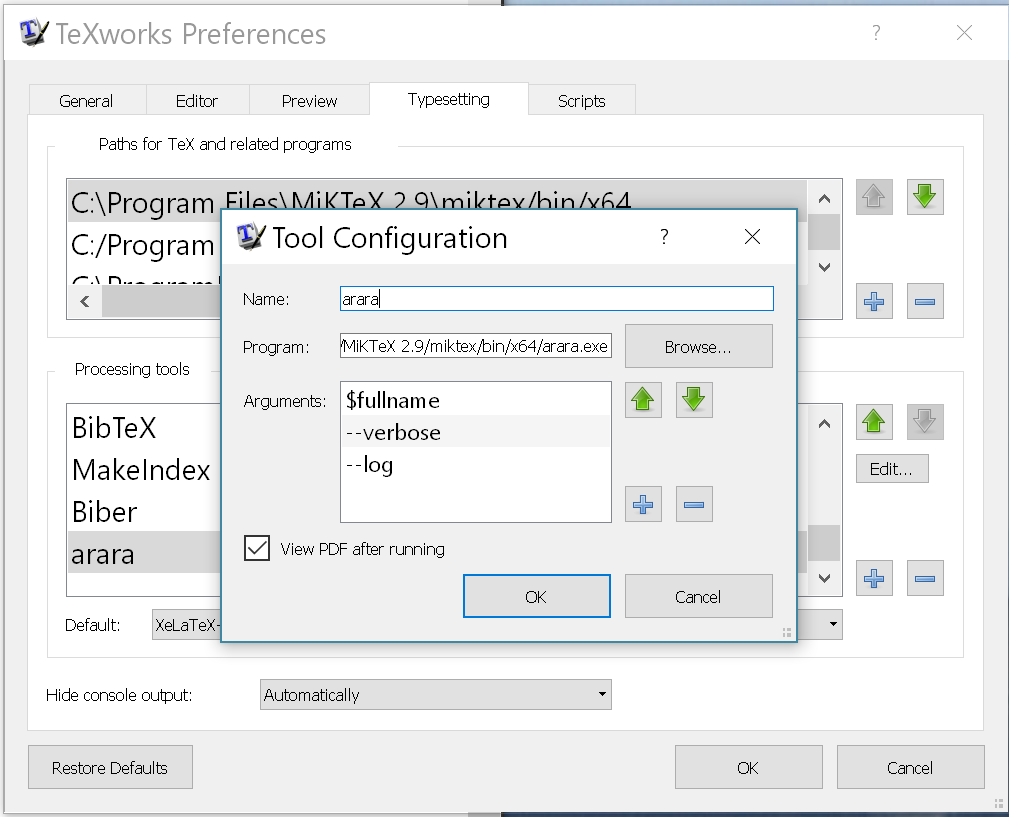
\includegraphics[scale=0.75]{../figs/arara.png}
\end{plScreen}
\vfill
\end{plSection}%{Typesetting}

%-----------------------------------------------------------------
%-----------------------------------------------------------------
\end{document}
%-----------------------------------------------------------------
